\documentclass[10pt,twocolumn]{article}

\usepackage[T1]{fontenc}
\usepackage{lmodern}
\usepackage{microtype}
\usepackage[a4paper,top=19mm,bottom=21mm,left=17mm,right=17mm,columnsep=7mm]{geometry}
\usepackage{amsmath,amssymb,amsthm,mathtools,bm}
\usepackage{booktabs,tabularx,array}
\usepackage{graphicx}
\usepackage{tikz}
\usetikzlibrary{arrows.meta,positioning,calc}
\usepackage{xcolor}
\usepackage{url}
\usepackage{placeins}
\usepackage{hyperref}
\usepackage[nameinlink,capitalise]{cleveref}
\usepackage{authblk}
\usepackage{balance}

\definecolor{linkblue}{HTML}{174A7E}
\definecolor{darkgreen}{HTML}{246B45}
\hypersetup{
  colorlinks=true,
  linkcolor=linkblue,
  citecolor=darkgreen,
  urlcolor=linkblue,
  pdftitle={CARMEN-Q: Causal Audit-Return Duality for Streaming Quantum Memory},
  pdfauthor={Javier Emilio Bazan Sanchez},
  pdfsubject={Exact causal audit-return bounds and reproducible quantum-memory benchmarks},
  pdfkeywords={quantum memory, causal benchmark, entanglement fidelity, information-disturbance}
}

\graphicspath{{../figures/}}
\setlength{\emergencystretch}{2em}
\setlength{\parindent}{1em}
\setlength{\parskip}{0pt}
\setlength{\columnsep}{7mm}
\raggedbottom
\renewcommand{\topfraction}{0.95}
\renewcommand{\dbltopfraction}{0.95}
\renewcommand{\textfraction}{0.05}
\renewcommand{\floatpagefraction}{0.75}
\renewcommand{\dblfloatpagefraction}{0.75}

\newtheorem{definition}{Definition}[section]
\newtheorem{theorem}[definition]{Theorem}
\newtheorem{proposition}[definition]{Proposition}
\newtheorem{lemma}[definition]{Lemma}
\newtheorem{corollary}[definition]{Corollary}
\theoremstyle{remark}
\newtheorem{remark}[definition]{Remark}
\newtheorem{limitation}[definition]{Limitation}

\newcommand{\Tr}{\operatorname{Tr}}
\newcommand{\id}{\mathbb{I}}
\newcommand{\ket}[1]{\lvert #1\rangle}
\newcommand{\bra}[1]{\langle #1\rvert}
\newcommand{\proj}[1]{\lvert #1\rangle\!\langle #1\rvert}
\newcommand{\PA}{P_{\mathrm A}}
\newcommand{\FR}{F_{\mathrm R}}
\newcommand{\Sscore}{S_{n,\lambda}}
\newcommand{\Cstream}{C^{\mathrm{stream}}_{n,\lambda}}
\newcommand{\Ccoll}{C^{\mathrm{coll}}_{\lambda}}
\newcolumntype{Y}{>{\raggedright\arraybackslash}X}

\newenvironment{takeaway}
  {\par\smallskip\noindent\begin{minipage}{\columnwidth}\small
   \color{linkblue}\rule{\columnwidth}{0.5pt}\par\smallskip
   \textbf{At a glance.}\enspace\color{black}}
  {\par\smallskip\color{linkblue}\rule{\columnwidth}{0.5pt}\end{minipage}\par\smallskip}

\title{{\normalsize\color{linkblue}\bfseries CARMEN-Q}\\[0.25em]
\textbf{Causal Audit--Return Duality for Streaming Quantum Memory}\\
\large An exact classical-memory frontier and a coherent one-qubit separation}
\author[1]{Javier Emilio Baz\'an S\'anchez}
\affil[1]{Facultad de Ciencias, Universidad Nacional Aut\'onoma de M\'exico, Mexico City, Mexico\\
\texttt{bazan@ciencias.unam.mx}}
\date{12 August 2026}

\begin{document}
\maketitle

\begin{abstract}
We introduce a two-branch benchmark for coherent memory in a sequential quantum process. A trusted verifier sends one half of each of $n$ independent EPR pairs through a device, requires every output to be committed before the next input is released, and sequesters those outputs. After the stream and the device's terminal-memory commitment, a hidden choice requests either (AUDIT) the parity of later computational-basis measurements on the references or (RETURN) joint recovery of all EPR pairs and visible reset of the terminal memory. For the explicit null class of arbitrary adaptive local instruments with unlimited classical memory and disposable within-slot ancillas, but no coherent state or entanglement persisting between slots, we prove the exact support
\[
\Cstream=max_{0\leq t\leq1}\left[
\frac{\lambda}{2}(1+t^n)+(1-\lambda)
\left(\frac{1+\sqrt{1-t^2}}2\right)^n\right].
\]
The reduction covers non-QND instruments and arbitrary transcript-conditioned joint recovery. At equal branch weight, the null is $3/4$ for every $n\geq2$, whereas one persistent coherent qubit attains $(\PA,\FR)=(1,1)$. A collective instrument retaining only a classical outcome has the strictly larger support
$\Ccoll=\tfrac12+\tfrac12\sqrt{\lambda^2+(1-\lambda)^2}$, isolating the causal cost of streaming. For $n\geq3$, the optimal classical strategy exhibits a first-order transition from recording nothing to an almost projective per-slot measurement. We supply a fixed-sample statistical certificate with explicit systematic allowances, conservative power planning, adversarial numerical checks, deterministic data and figures, and a hardware-facing protocol. The result is a trusted-interface temporal quantum-memory witness, not a device-independent claim, a proof of global erasure, or evidence for a preferred interpretation of quantum mechanics.
\end{abstract}

\noindent\textbf{Keywords:} quantum memory; multitime quantum processes; information--disturbance; entanglement fidelity; reversible computation; causal benchmarks.


\section{Introduction}

A memory is operationally quantum only when coherence carried across time changes what a process can do. Merely observing a reversible circuit, a final interference fringe, or an auxiliary register returned to zero is not enough: a known closed circuit can be compiled into an endpoint-equivalent channel that never instantiates the advertised intermediate record. The scientific question therefore needs an access model and a comparison class, not interpretive vocabulary.

We study a streamed task with two incompatible late uses of one committed process. The verifier supplies fresh entangled carriers one at a time and permanently removes each returned carrier from the device. Only after the final slot does a hidden choice ask the committed memory either to reveal a temporal predicate or to help reverse the disturbance created while learning it. The predicate is the parity of $n$ later reference outcomes. The reversal target is global entanglement fidelity of all $n$ returned carriers. These endpoints force the same prefix to be useful as a record and reversible as a coherent process.

The ingredients are familiar. Information acquisition competes with disturbance \cite{banaszek2001fidelity}; read-versus-return tasks appear in quantum sealing \cite{kimmel2019seals}; late path-versus-phase games quantify operational duality \cite{bagan2018duality}; and parity discrimination has a long history in quantum cryptography \cite{bennett1996parity}. Multitime process formalisms distinguish quantum, classical, and memoryless transmission across slots \cite{chiribella2009networks,pollock2018processes,taranto2024hierarchy}. Sequential random-access tasks and bounded-memory channel discrimination already witness quantum memory under other scores and assumptions \cite{roy2024semidevice,ohst2026memory}. Our claimed contribution is not any of these ingredients alone.

For a precisely declared classical-memory comb, we derive the complete audit--return support function. The proof first removes arbitrary non-QND output dynamics through a flagged entanglement-fidelity bound. Causal factorisation then turns both the posterior parity bias and the maximum return fidelity into products along every refined classical path. Adaptation becomes an average of deterministic strength profiles, and a convexity argument shows that equal local strengths attain the optimum. This supplies an exact causal tensorisation rather than a symmetric ansatz.

Three consequences make the result experimentally legible. First, at the balanced point the unlimited adaptive classical-memory score is $3/4$ for every stream length $n\geq2$. Second, allowing the carriers to be processed collectively before producing a classical record raises the score to $(1+1/\sqrt2)/2$, so sequestration is a physical resource restriction rather than cosmetic timing. Third, one coherent accumulator qubit reaches unit score and visibly resets in RETURN. The benchmark therefore compares three resource classes on the same task:
\[
\text{streaming classical memory}
\;<\;
\text{collective classical record}
\;<\;
\text{one coherent temporal qubit}
\]
for every nontrivial support direction, with the final inequality understood at the algebraic point.

We accompany the theorem with a fixed-sample statistical rule, a preregistration template, mandatory shortcut controls, deterministic frontier data, and a replaceable phenomenological error model. The goal is a benchmark that can be falsified. A positive result rejects the declared classical-memory interface. It does not identify a unique microscopic implementation, certify an unrestricted hidden device, prove deletion of inaccessible environmental records, or support claims about observers or alternate worlds.

\subsection{Contributions}

The paper provides:
\begin{enumerate}
  \item an operational AUDIT/RETURN task with immediate output sequestration and a terminal-memory commitment;
  \item an exact theorem for arbitrary adaptive, non-QND, classical-memory streaming instruments;
  \item closed forms, a first-order strategy transition for $n\geq3$, and a strict collective-classical comparator;
  \item an explicit one-qubit coherent strategy attaining perfect audit and return;
  \item a conservative finite-statistics certificate with systematic-error and null-model slack;
  \item reproducible analytic and numerical validation, planning data, controls, and implementation guidance.
\end{enumerate}

All novelty language is qualified by the dated literature audit. The safe claim is the exact streamed parity-audit versus global-entanglement-return frontier and its resource separation, to our knowledge---not weak measurement, parity processing, delayed choice, reversible computation, or quantum-memory witnessing in general.

\section{Scope, evidence levels, and adjacent literature}

\subsection{Epistemic firewall}

We distinguish four levels of statement throughout:

\begin{enumerate}
  \item \textbf{Operational:} specified coherent evolutions yield an interference signal and controls do not.
  \item \textbf{Model-relative historical:} components of a declared decomposition carry different internal records at intermediate times.
  \item \textbf{Interpretive:} one may describe those components using a preferred interpretation of quantum mechanics.
  \item \textbf{Unsupported:} the experiment accesses a pre-existing macroscopic alternative world or establishes a unique ontology.
\end{enumerate}

Only the first level is directly measured. The second follows from a validated model and declared tensor decomposition. The third is underdetermined by shared unitary predictions. The fourth is outside the protocol.

\subsection{Known ingredients}

Relative-state language and decoherence motivate discussions of correlated components and records \cite{everett1957relative,zurek2003decoherence}. Consistent-histories methods describe sequences and their decoherence functionals \cite{griffiths1984consistent,paz1993environment}, although alternatives that are deliberately recombined are not simultaneously a classical consistent family. Reversible computation supplies compute--copy-or-phase--uncompute constructions \cite{bennett1973logical}. Wave--particle duality and quantum erasure quantify the loss and conditional recovery of interference when path information exists \cite{englert1996fringe,kim2000delayed}. Measurement reversal and error-correction demonstrations establish that selected measurement interactions can be undone under controlled conditions \cite{katz2008reversal,schindler2013undoing}.

For multitime structure, quantum combs and process tensors treat an experiment as a process with intervention slots rather than as a single endpoint channel \cite{chiribella2009networks,pollock2018processes,hoffreumon2021multiround}. Quantum causal discovery makes interventions central to the distinction between correlation and causation \cite{giarmatzi2018causal}. Temporal studies can diagnose instrument-specific memory effects, bound effective environment dimension, and, under stronger assumptions, certify a quantum memory without trusting its implementation \cite{guo2021memory,vieira2024dimension,sekatski2023memory}. A January 2026 preprint reports a trapped-ion proof of principle for device-independent two-time memory certification \cite{santos2026deviceindependent}; its peer-review status at our cutoff is provisional.

Wigner-friend-inspired protocols show how a small physical record can play the functional role of an internal observer, including explicit analyses of memory erasure \cite{frauchiger2018quantum,proietti2019observer,bong2020strong,elouard2021erasing}. These works do not place a conscious human observer in coherent superposition. The memory-erasure result is a particularly direct antecedent and prevents a novelty claim based merely on a friend acquiring and then losing a record.

Quantum zero-knowledge proof systems establish rigorous ways for a verifier to learn validity without learning a witness, including QMA, classical-verifier protocols for quantum computations, non-destructive state proofs, and superposition-secure transcript models \cite{broadbent2016qma,vidick2020classical,colisson2025nondestructive,coladangelo2026mpc}. Their security definitions are computational or information-theoretic statements about simulators and adversaries. Our zero-record criterion instead asks whether physical residual systems remain correlated with distinctions inside a predicate class. The analogy is generative but not an equivalence.

Quantum algorithmic measurements (QUALMs) provide a complexity-theoretic language for experimental access and exhibit tasks with exponential separations between coherent and incoherent access \cite{aharonov2022qualm}. Computational mechanics supplies irreducible predictive-memory measures, and quantum models or adaptive agents can reduce memory costs for selected stochastic processes \cite{gu2012complexity,elliott2022agents}. These results suggest the right form of a future originality claim: not that a circuit used superposition, but that a precisely defined historical-certification task has a provable resource separation.

\subsection{Evidence and novelty discipline}

We classify claims as known results, derivations, numerical observations, conjectures, or open objectives. The accompanying literature review is a scoping review rather than a PRISMA systematic review. Several directly adjacent manuscripts appeared as 2026 preprints and remain provisional at the cutoff date. Consequently, the phrase ``not found in this search'' is never promoted to ``never proposed.'' A priority claim requires database-complete searches, forward and backward citation tracing, and specialist review.

The elementary history--predicate--uncompute circuit is not new. Generic memory--visibility inequalities are also heavily constrained by existing complementarity and channel-recovery results \cite{englert1996fringe,kretschmann2008information}. The candidate open intersection is the joint task of causal-memory certification, within-predicate zero-record leakage, and subsequent recoherence under an explicit access model.

\subsection{Adversarial novelty map}

Table~\ref{tab:novelty} records which intuitive headlines are already occupied. It is deliberately stricter than a conventional motivation section.

\begin{table}[ht]
\centering
\caption{Adjacency audit at the 12 August 2026 cutoff. The final row is a candidate research task, not an established priority claim.}
\label{tab:novelty}
\small
\begin{tabularx}{\textwidth}{@{}>{\raggedright\arraybackslash}p{0.23\textwidth}Y Y@{}}
\toprule
Candidate headline & Existing territory & Remaining requirement \\
\midrule
Compute a predicate and erase work & Reversible computation and phase kickback & No novelty without a new access or resource theorem \\
Erase an internal observer's memory & Wigner-friend memory erasure is explicit prior work & Certify causal memory and nonvacuous final privacy \\
Bound memory by temporal data & Process-tensor and memory-dimension witnesses exist & Combine the witness with a later coherent inverse \\
Hide a quantum witness or transcript & Quantum zero-knowledge protocols cover strong adversarial models & Relate simulator security to physical final-record decoupling \\
Show coherent experimental advantage & QUALMs already give exponential separations for other tasks & Prove a separation for the zero-record task itself \\
Trade objectivity against recovery & Darwinism, encoding transitions, and QEC tradeoffs are active & Only a narrower operational theorem may remain \\
Causal memory + predicate-only disclosure + final decoupling + recoherence & No single primary source located by the bounded search & Formal anti-shortcut model and nontrivial theorem still required \\
\bottomrule
\end{tabularx}
\end{table}

\subsection{Direct 2026 priority risks}

The current literature makes interpretation-led framing especially risky. Three January 2026 preprints use inter-branch communication language, compile Wigner-friend-style message circuits, or benchmark them on superconducting processors \cite{violaris2026branches,altman2026wigner,cogburn2026interbranch}. Another January preprint studies approximate records, decoherence, recoherence, and recovery in long isolated histories \cite{strasberg2026records}. These manuscripts are not treated as settled peer-reviewed results, but they are direct priority evidence against presenting branch communication, memory erasure, or generic recoherence as new.

Quantum Darwinism formalises redundant proliferation of classical records, and models already connect redundant objective information with consistent histories and quantum encoding \cite{blumekohout2006darwinism,riedel2016objective,ferte2024transition}. A March 2026 peer-reviewed model further distinguishes approximate decoherent histories from the redundant records associated with objectivity \cite{ferte2026histories}. A preprint posted eight days before our cutoff claims an exact QEC--Darwinism tradeoff and a model-independent no-go statement \cite{maity2026tradeoff}. Its generality requires independent scrutiny, but its existence makes objectivity versus recoverability a poor novelty headline.

Thermodynamic erasure is also not an empty intersection. Complexity-constrained quantum thermodynamics derives work--complexity tradeoffs for reset \cite{munson2025complexity}, while microscopic measurement models study records, reset, finite-time control, and work \cite{latune2025measurement}. Our inverse is logically reversible; assigning \(k_BT\ln2\) to every uncomputed bit would conflate uncomputation with blind erasure.

\subsection{Macroscopic scale and nonunitarity}

Matter-wave experiments have extended coherent interference to increasingly massive molecules and nanoparticles, including a 2026 sodium-nanoparticle result \cite{pedalino2026nanoparticle}. This calibrates centre-of-mass coherence, not reversible control of a macroscopic internal observer and its environment. Objective-collapse models make parameterised predictions and are experimentally constrained, including by a March 2026 XENONnT spontaneous-radiation search \cite{bassi2013collapse,nimmrichter2014optomechanical,arnquist2022majorana,aprile2026collapse}. An unexplained visibility loss in the present protocol would first indicate an incomplete noise or control model; it would not by itself identify fundamental nonunitarity.

\subsection{Conservative novelty statement}

The dated search found primary literature for every clause separately but did not locate a protocol that jointly imposes: (i) an interventional lower bound on causal memory, (ii) disclosure limited to a non-injective predicate, (iii) final decoupling of every other accessible history record, (iv) recovered interference, and (v) an explicit shortcut class. This is a bounded negative search result, not proof of absence. A first submission must add citation-network traversal, subscription-database searches, patent and thesis checks, and independent specialist review before using a phrase such as \emph{to our knowledge}.

\section{Operational model}
\label{sec:model}

Fix $n\geq1$. At slot $i$, a trusted verifier prepares
\[
\ket{\Phi}_{R_iA_i}=\frac{\ket{00}+\ket{11}}{\sqrt2},
\]
sends $A_i$ to the device, receives $B_i$, and sequesters $B_i$ before releasing $A_{i+1}$. After the last output, the device commits a terminal memory port $M$ to the verifier. A hidden coin then selects one branch.

\paragraph{AUDIT.}
The verifier measures every $R_i$ in $Z$, obtaining independent uniform bits $X_i$, and decodes from $M$ a guess for
\[
Z=X_1\oplus\cdots\oplus X_n.
\]
The sequestered $B_i$ are unavailable. Let $\PA$ be the success probability.

\paragraph{RETURN.}
The verifier applies a fixed joint decoder to $M B_1\cdots B_n$ and accepts with
\[
\Pi_{\mathrm R}=\proj{0}_M\otimes
\bigotimes_{i=1}^n\proj{\Phi}_{R_iB_i}.
\]
Let $\FR$ be the acceptance probability. The visible reset $M=0$ does not imply deletion of any inaccessible purification of a classical record.

For $0\leq\lambda\leq1$, define the support score
\[
\Sscore=\lambda\PA+(1-\lambda)\FR.
\]
The balanced benchmark uses $\lambda=1/2$.

\subsection{Adaptive classical-memory streaming null}

The null may use arbitrary finite classical memory and shared randomness. In slot $i$, conditional on the earlier classical history $h=k_{<i}$, it applies an arbitrary instrument
\[
\{\mathcal N^{(i,h)}_{k_i}:A_i\rightarrow B_i\}_{k_i}.
\]
It may create and discard arbitrary within-slot quantum ancillas. It may not retain a coherent system across the slot boundary, begin with entanglement shared between slot ancillas, revisit a committed $B_i$, or receive a $B_i$ in AUDIT. In RETURN, the full classical transcript may control an arbitrary joint recovery on all sequestered outputs.

After refining all classical random seeds and outcomes, every leaf transcript $k=(k_1,\ldots,k_n)$ has a conditional channel that factorises over slots. For computational-basis inputs $x=(x_1,\ldots,x_n)$, its likelihood is
\begin{equation}
p(k|x)=\prod_{i=1}^n p_i(k_i|x_i,k_{<i}).
\label{eq:factor}
\end{equation}
This factorisation is the mathematical null. The experiment must support it through timing and isolation evidence; the score alone cannot enforce a laboratory boundary.

\subsection{Local audit strength and return curve}

At a realised prefix $h$, define
\[
r_i(k_i|h)=\frac{p_i(k_i|0,h)+p_i(k_i|1,h)}{2}
\]
and, when $r_i>0$, define a signed posterior bias by
\begin{equation}
s_i\delta_i=
\frac{p_i(k_i|0,h)-p_i(k_i|1,h)}
{p_i(k_i|0,h)+p_i(k_i|1,h)},
\qquad 0\leq\delta_i\leq1.
\label{eq:bias}
\end{equation}
The one-slot return curve is
\begin{equation}
f(t)=\frac{1+\sqrt{1-t^2}}{2}.
\label{eq:fcurve}
\end{equation}
Here $t=0$ extracts no computational-basis information and preserves an EPR pair perfectly; $t=1$ permits a perfect bit record and leaves entanglement fidelity $1/2$.

\subsection{A saturating null family}

For any $t_i\in[0,1]$, the binary diagonal instrument
\[
K^{(i)}_0=
\begin{pmatrix}
\sqrt{(1+t_i)/2}&0\\0&\sqrt{(1-t_i)/2}
\end{pmatrix},\quad
K^{(i)}_1=
\begin{pmatrix}
\sqrt{(1-t_i)/2}&0\\0&\sqrt{(1+t_i)/2}
\end{pmatrix}
\]
produces local audit bias $t_i$ and return fidelity $f(t_i)$. The transcript parity is the optimal AUDIT guess and identity recovery saturates the RETURN expression derived below.

\section{Exact frontiers and resource separation}
\label{sec:results}

We first state the full frontier, then unpack its consequences. Readers interested mainly in the experimental message can read the highlighted balanced case and the resource comparison; all proof details are in \cref{app:proofs}.

\begin{theorem}[Streaming parity audit--return frontier]
For the adaptive classical-memory null in \cref{sec:model}, including arbitrary non-QND local instruments and arbitrary transcript-conditioned joint recovery,
\begin{small}
\begin{align}
\Cstream
&=\max_{0\leq t_1,\ldots,t_n\leq1}
\left[
\frac{\lambda}{2}\left(1+\prod_{i=1}^n t_i\right)
+(1-\lambda)\prod_{i=1}^n f(t_i)
\right] \label{eq:productfrontier}\\
&=\max_{0\leq t\leq1}
\left[
\frac{\lambda}{2}(1+t^n)+(1-\lambda)f(t)^n
\right].
\label{eq:frontier}
\end{align}
\end{small}
The bound is attainable by independent weak diagonal instruments.
\end{theorem}

The proof has three moves. First, a Choi-positivity lemma bounds recoverable EPR fidelity using only basis-state likelihoods. Second, causality makes both the posterior parity bias and the return fidelity factorise across slots. Third, convexity shows that an optimal strategy uses the same strength in every slot. This is why the many-instrument optimisation collapses to the single variable $t$ in \eqref{eq:frontier}.

\begin{corollary}[Balanced null]
For $n\geq2$ and $\lambda=1/2$,
\[
\Cstream=\frac34.
\]
The least-disturbing optimum is $t=0$: the null learns no parity beyond chance and returns every EPR pair.
\end{corollary}

\begin{takeaway}
At $\lambda=1/2$, a classical-memory device cannot improve the score by measuring weakly: for every $n\geq2$, its best choice is to keep no record, guess parity, and return the EPR pairs. The ceiling is therefore $\tfrac12(\tfrac12+1)=\tfrac34$.
\end{takeaway}

\subsection{Closed forms and the strategy transition}

For one slot,
\[
C^{\mathrm{stream}}_{1,\lambda}
=\frac12+\frac12\sqrt{\lambda^2+(1-\lambda)^2}.
\]
For two slots,
\begin{equation}
C^{\mathrm{stream}}_{2,\lambda}=
\begin{cases}
1-\lambda/2,&0\leq\lambda\leq1/2,\\[1mm]
\lambda/2+\lambda^2/(3\lambda-1),&1/2<\lambda\leq1.
\end{cases}
\label{eq:n2}
\end{equation}
The optimal strength grows continuously from zero at $\lambda=1/2$.

The weighted game reveals additional structure. For $n\geq3$, the optimal classical strategy changes discontinuously as AUDIT becomes more important. Let $z_n$ be the unique solution
\begin{equation}
(1-z_n)(1+z_n)^{n-1}=1,\qquad
z_n\in\left(\frac{n-2}{n},1\right).
\label{eq:zn}
\end{equation}
Then
\begin{equation}
\lambda_c(n)=
\frac{1}{1+2^{n-2}z_n^{(n-2)/2}(1-z_n)}.
\label{eq:lambdac}
\end{equation}
Below $\lambda_c$, the optimum is $t=0$. At $\lambda_c$, it ties a finite-strength branch, so the optimal strength jumps discontinuously. For $n=3,4,5$, respectively, $(\lambda_c,t_c)$ is approximately $(0.6248,0.9717)$, $(0.6495,0.9962)$, and $(0.6589,0.9993)$. Moreover $\lambda_c(n)\to2/3$ from below. The optimal null thus changes from recording nothing to recording each slot almost projectively rather than moving through a broad weak-measurement phase.

\subsection{Collective classical-record comparator}

Now remove streaming sequestration and allow one joint instrument on all carriers, while requiring that only a classical outcome survives the commit point.

\begin{proposition}[Collective classical record]
For every $n$,
\begin{equation}
\Ccoll=\frac12+\frac12\sqrt{\lambda^2+(1-\lambda)^2}.
\label{eq:collective}
\end{equation}
For $n\geq2$ and $0<\lambda<1$, this is strictly larger than $\Cstream$.
\end{proposition}

A weak measurement of the two parity subspaces attains \eqref{eq:collective}. This comparator still retains only a classical outcome; its advantage comes from seeing all carriers together. It therefore measures exactly what is lost when the apparatus must operate as a stream.

\subsection{One coherent qubit closes the gap}

Initialise a memory qubit $M=\ket0$. In slot $i$, apply $\mathrm{CNOT}_{A_i\rightarrow M}$ and return $A_i$. After the final slot, commit $M$.
In AUDIT, measuring $M$ in $Z$ gives the parity of the later $Z$ measurements on the references. In RETURN, applying $\mathrm{CNOT}_{B_i\rightarrow M}$ for every sequestered carrier uncomputes $M$ to $\ket0$ and exactly restores all EPR pairs. Thus $(\PA,\FR)=(1,1)$. The operational resource is a coherent temporal accumulator, not an observer or an interpretation of quantum mechanics.

\section{Statistical certificate and experimental protocol}
\label{sec:protocol}

The theorem gives a probability bound; an experiment needs a decision rule. The rule below separates three ingredients that are often conflated: sampling uncertainty, measured bias in each branch, and uncertainty in whether the laboratory really implements the theoretical null.

\subsection{Fixed-sample certificate}

Let $(K_{\mathrm A},N_{\mathrm A})$ and $(K_{\mathrm R},N_{\mathrm R})$ be successes and fixed trials in the two branches. Define
\[
\widehat S=\lambda\frac{K_{\mathrm A}}{N_{\mathrm A}}
+(1-\lambda)\frac{K_{\mathrm R}}{N_{\mathrm R}}.
\]
For independent Bernoulli trials, the one-sided weighted Hoeffding radius is
\begin{equation}
r_\alpha=
\sqrt{\frac12\left(
\frac{\lambda^2}{N_{\mathrm A}}+
\frac{(1-\lambda)^2}{N_{\mathrm R}}
\right)\log\frac1\alpha}.
\label{eq:hoeffding}
\end{equation}
Before observing outcomes, let $\delta_{\mathrm A}$ and $\delta_{\mathrm R}$ upper-bound possible upward bias in the two estimators, and let $\delta_{\mathrm{null}}$ enlarge the theoretical null for source, isolation, and interface uncertainty. We certify incompatibility with the declared classical-memory null only if
\begin{equation}
\widehat S-\lambda\delta_{\mathrm A}
-(1-\lambda)\delta_{\mathrm R}-r_\alpha
>\Cstream+\delta_{\mathrm{null}}.
\label{eq:certificate}
\end{equation}
Under independent fixed-sample trials, the false-positive probability is at most $\alpha$. Choosing $n$ or $\lambda$ after seeing data, optional stopping, or selecting the best of several lengths requires a different analysis.

For an alternative score $S_{\mathrm{alt}}$, define
\[
g=S_{\mathrm{alt}}-\lambda\delta_{\mathrm A}
-(1-\lambda)\delta_{\mathrm R}
-\Cstream-\delta_{\mathrm{null}}.
\]
If $g\leq0$, no amount of data certifies the claim under those allowances. If $g>0$, fixed sample sizes satisfying $r_\alpha+r_\beta<g$ guarantee power at least $1-\beta$ by a second Hoeffding bound. The implementation allocates trials asymptotically as $N_{\mathrm A}:N_{\mathrm R}=\lambda:(1-\lambda)$.

\subsection{Commitment and branch timing}

A valid trial follows the left-to-right order of \cref{fig:protocol}. The verifier first prepares and independently characterises the EPR sources. It releases $A_i$ only after $B_{i-1}$ has entered trusted sequestration and, after receiving $B_n$, requires delivery of the terminal memory port $M$. Only then is the hidden AUDIT/RETURN choice generated. The preregistered branch decoder and binary acceptance measurement are applied, and every loss or exclusion is recorded under a predeclared rule. The branch may be randomised per trial, but the final branch counts and stopping rule must be fixed or analysed with a sequentially valid method.

\subsection{Mandatory shortcut controls}

These controls are part of the scientific claim, not optional diagnostics. Deliberately dephasing the persistent carrier should remove the coherent advantage, whereas making a strong classical record should improve AUDIT while lowering global RETURN. Removing sequestration should recover the collective curve in \eqref{eq:collective}; allowing the device to revisit an earlier $B_i$ should likewise expose why the causal boundary matters. Decoder controls replace the coherent inverse by identity or by a mismatched inverse. Independent source and measurement calibration must bound false EPR acceptance and parity bias, and a blind-choice control must test whether branch information leaks before commitment. Finally, a side-channel audit must bound coherent transfer through buses, pulse tails, clocks, resonators, unused levels, and shared ancillas.

The null does not forbid inaccessible erasure environments. Consequently, visible reset of $M$ is a reproducibility and wiring check, not a certificate that every physical copy of a classical transcript has vanished.

\subsection{Reproducible analysis interface}

The public command-line tool evaluates the exact bound, plans trial counts, and applies the fixed-sample rule through three strict-JSON commands:
\begin{small}
\begin{verbatim}
carmenq bound --steps 8
carmenq plan --steps 8 --forecast-model
carmenq analyse --steps 8 \
  --audit-successes 9700 --audit-trials 10000 \
  --return-successes 9500 --return-trials 10000
\end{verbatim}
\end{small}
Systematic allowances, $\alpha$, $\beta$, and null slack are command-line inputs and appear in the output. An example preregistration records the terminal port, source calibration, decoder, exclusions, controls, and stopping rule.

\section{Numerical validation and forecast}
\label{sec:numerics}

The theorem is analytic. Computation is used to attack the derivation, expose transitions, and convert a declared noise law into a shot budget; it is not used as a substitute for the proof.

\subsection{Adversarial theorem checks}

Independent scripts checked:
\begin{itemize}
  \item the one- and two-slot closed forms and transition equations through $n=12$;
  \item random product likelihoods against the flagged recovery inequality;
  \item random collective likelihood tables against \eqref{eq:collective};
  \item the exact coherent-accumulator circuit;
  \item asymmetric local strengths and fully adaptive outcome trees for $n=2,\ldots,5$.
\end{itemize}
The maximum numerical excess over the streaming theorem was $6.52\times10^{-14}$ for adaptive trees and $3.53\times10^{-14}$ for asymmetric products, consistent with numerical precision. The smallest tested collective-classical gap was positive. These checks do not prove the theorem or priority; they are regression tests against algebraic and implementation errors.

The release suite contains 25 automated tests. It verifies exact supports, transition behaviour, conservative systematic handling, fixed-sample planning, strict JSON output, deterministic simulation, and byte-stable same-environment figures and data.

\subsection{Transparent forecast model}

For planning only, we use the replaceable phenomenological law
\begin{equation}
\PA(n)=\frac{1+c_0c^n}{2},\qquad
\FR(n)=f_0 f^n.
\label{eq:forecast}
\end{equation}
The committed defaults are $c_0=f_0=0.995$, $c=0.998$, and $f=0.997$. They are illustrative logical-operation factors, not hardware calibration.

With $\lambda=1/2$, $\alpha=0.01$, target power $0.9$, $0.005$ systematic allowance in each branch, and $0.005$ null slack, the model's robust plan remains feasible through $n=143$ and becomes infeasible at $n=144$. The unadjusted expected score first crosses the $3/4$ asymptotic streaming null at $n=151$. Near the robust boundary the conservative Hoeffding shot count diverges rapidly, making uncertainty accounting more important than small circuit optimisations.

At $n=8$, a declared alternative $(\PA,\FR)=(0.97,0.95)$ under the same allowances needs 84 trials per branch for the Hoeffding guarantee ($\alpha=0.01$, power at least $0.9$). If 9700 of 10000 AUDIT trials and 9500 of 10000 RETURN trials succeed, the adjusted one-sided lower score is approximately $0.9443$, exceeding the enlarged $0.755$ null by approximately $0.1893$.

\begin{figure}[ht]
\centering
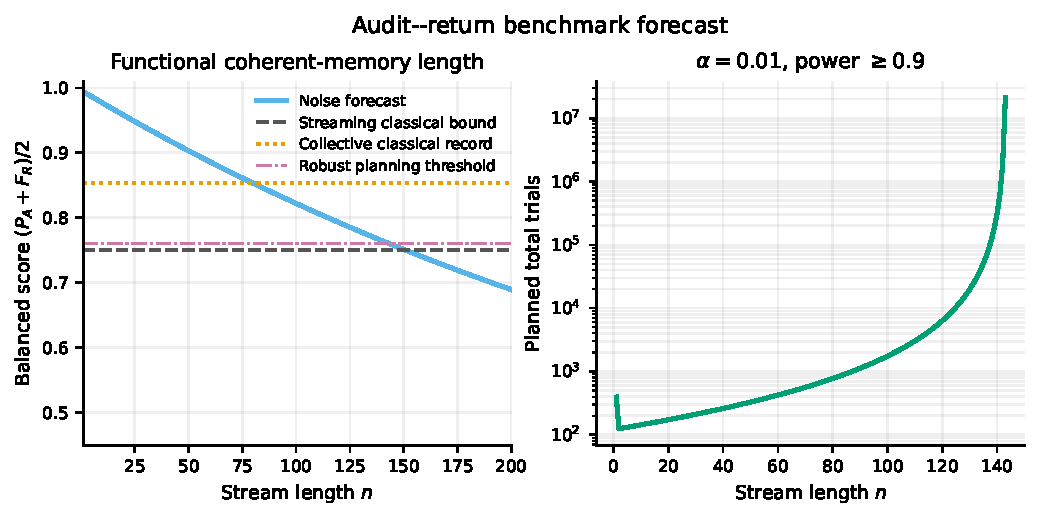
\includegraphics[width=\textwidth]{audit_return_benchmark.pdf}
\caption{Illustrative forecast from \eqref{eq:forecast}. Left: balanced score against the streaming, collective-classical, and robust planning thresholds. The one-slot streaming point is higher than the $n\geq2$ plateau. Right: conservative total trial count from \eqref{eq:hoeffding}; infeasible lengths are omitted. These curves are not hardware predictions.}
\label{fig:forecast}
\end{figure}
\FloatBarrier

\subsection{Functional coherent-memory length}

We define the \emph{certifiable functional coherent-memory length} as the largest preregistered $n$ for which \eqref{eq:certificate} is satisfied under a declared familywise testing rule. Unlike a bare $T_2$, it asks a memory to retain a temporal predicate and later participate in coherent global return. It remains benchmark-specific: changing the predicate, branch scores, or sequestration interface changes the resource being measured.

\section{Experimental feasibility}
\label{sec:feasibility}

\subsection{Minimal logical circuit}

The honest coherent device needs one persistent qubit and $n$ streamed carrier interactions. In the ideal binary implementation:
\begin{enumerate}
  \item the source creates $n$ EPR pairs;
  \item the device applies one $\mathrm{CNOT}_{A_i\rightarrow M}$ per slot;
  \item a trusted switch routes every returned $B_i$ to storage inaccessible to the device;
  \item after the terminal memory is committed, AUDIT measures $M$ and the $R_i$ in $Z$;
  \item RETURN applies $n$ inverse CNOTs from $B_i$ to $M$, then Bell-tests every $R_iB_i$ and tests $M=0$.
\end{enumerate}
The logical depth inside the untrusted device is one two-qubit gate per slot. The recovery station has $n$ further two-qubit gates and $n$ Bell analysers. The global RETURN event is deliberately stringent: every pair and the terminal reset must pass in the same trial.

\subsection{The hard part is the interface}

Gate counts are modest; causal enforcement is not. An implementation needs all of:
\begin{itemize}
  \item a switch or transport geometry that proves $B_i$ left the device before $A_{i+1}$ arrived;
  \item storage of every $B_i$ with sufficiently low loss and dephasing for the later joint decoder;
  \item a terminal port that transfers $M$ without revealing the branch choice;
  \item calibrated suppression of coherent paths that cross slot boundaries outside the charged memory;
  \item a random branch generator and control electronics whose timing cannot leak into the device.
\end{itemize}
A hidden bus mode or coherent pulse tail is not ``noise'' under the theorem: it is precisely a quantum-memory resource that moves the apparatus outside the null. Such a side channel may still produce a valid positive witness of some coherent memory, but it prevents attributing the result to the nominated memory qubit.

\subsection{Candidate platforms}

Superconducting circuits can combine fast controlled gates, a dedicated memory or bus mode, and microwave routing, but resonator and control-line remnants require an explicit side-channel budget. Trapped ions offer long-lived internal memories and high-quality entangling gates, while physical sequestration is naturally expressed through shuttling, zones, or trusted spectator isolation. Neutral-atom arrays offer reconfigurable geometry and parallel entanglement tests, with loss treatment needing preregistration. Photonic time bins coupled to a matter memory naturally realise a stream, but source loss, storage loss, and postselection are central risks.

The protocol does not select a platform by headline fidelity alone. The decisive platform metric is whether the access model can be made credible and independently audited.

\subsection{Staged demonstration}

\begin{enumerate}
  \item \textbf{$n=2$ logical demonstration:} verify the coherent point and the dephased-memory control.
  \item \textbf{Classical frontier:} implement weak diagonal instruments and recover the predicted support curve as $\lambda$ varies.
  \item \textbf{Causal separation:} compare enforced streaming with the collective-access control on the same hardware.
  \item \textbf{Length scaling:} preregister $n$ values and report simultaneous confidence intervals or corrected tests.
  \item \textbf{Independent interface audit:} characterise leakage channels without using the primary score data.
\end{enumerate}

\subsection{Kill criteria}

The flagship claim must be reduced or abandoned if:
\begin{enumerate}
  \item the theorem's classical-path factorisation does not match the stated experimental null;
  \item an adaptive classical strategy exceeds \eqref{eq:frontier};
  \item the branch choice or sequestered carriers become accessible before commitment;
  \item postselection or loss rules can condition the score on hidden outcomes;
  \item source correlations invalidate independence of the $X_i$;
  \item the reported score uses average pair fidelity instead of the global RETURN event;
  \item an earlier theorem is found that directly specialises to the full interface and support;
  \item systematic allowances needed to defend the access model erase the statistical gap.
\end{enumerate}
Any of these outcomes would still leave useful calibration or pedagogy, but not the claimed exact resource witness.

\section{Discussion and conclusions}

The central positive result is modest but exact: a quantum process may create distinguishable internal records, compute a property from them, convert that property to phase, and uncompute every controlled record while retaining an interferometric effect. Internal processing and conditional action do not introduce a new fundamental source of decoherence. What matters is whether history-dependent information remains outside the inverse and whether accumulated control errors preserve the required phase.

The central negative result is equally important: the same endpoint channel can be implemented without the advertised internal history. Therefore, a final interference fringe cannot certify an agent, a memory depth, or a unique temporal narrative. The direct-phase control is supposed to agree. Historical authenticity becomes a scientifically distinct question only after an access model introduces intervention times, late inputs, locality, black-box dynamics, or resource bounds.

Zero record gives a useful accounting rule. It is not enough to set a named memory qubit to zero; every residual system must be checked for distinctions that the allowed predicate does not reveal. Conditional mutual information captures this within-predicate requirement, provided the predicate is non-injective. The four-history benchmark exists specifically to prevent a formally correct but vacuous privacy score.

The analytic late-challenge protocol moves one step beyond a static ancilla. A classical response at a later time depends on information acquired before the challenge, and a bounded classical-memory comparison gives a quantitative success limit. The coherent phase variant uses the same response function, but its endpoint task is not the classical random-access score, and the current simulator does not model challenge independence. Both statements remain architecture-relative. If a shortcut device can access the history label when the response is produced, it can insert the phase directly. A publishable causal advance requires a witness or interactive task that makes the forbidden access operational rather than rhetorical.

Three research directions are defensible. First, process-tensor and temporal-correlation tools may yield a targeted memory-dimension witness compatible with a later inverse. Second, quantum-algorithmic-measurement methods may establish a coherent-versus-incoherent query separation for a black-box history property. Third, simulator-based quantum zero-knowledge ideas may inspire a composable definition in which a verifier learns a predicate while any allowed residual view is simulable from that predicate alone. None of these results is claimed here.

The programme should be discontinued as a distinct research framing if every candidate task compiles to a known phase oracle under the same access assumptions, if memory cannot be causally witnessed, or if no new resource bound or experimentally distinguishable prediction results. A rigorous negative result would still be valuable: it would identify exactly why reversible internal narrative adds no operational resource beyond coherent computation.

In its present form, the project is a completed baseline rather than a completed research field. It supplies definitions, no-go statements, reference circuits, controls, reproducible numerics, and a falsifiable next target. Its scientific claim is not that quantum mechanics exposes alternative universes. It is that the boundary between a record-rich internal process and its recoverable coherence can be formulated as a precise causal-information task, and that any stronger claim must survive endpoint equivalence, transcript accounting, and explicit comparison models.


\appendix
\section{Proofs}
\label{app:proofs}

\subsection{Flagged entanglement-recovery lemma}

\begin{lemma}
Let $\mathcal N_k:A\rightarrow B$ be a trace-nonincreasing CP map, $\dim A=D$, and
\[
p(k|x)=\Tr\mathcal N_k(\proj{x})
\]
in a fixed orthonormal basis. For any recovery channel $\mathcal R_k:B\rightarrow A$, its unnormalised contribution to the maximally entangled-state fidelity satisfies
\begin{equation}
F_k\leq\frac1{D^2}\left(\sum_x\sqrt{p(k|x)}\right)^2.
\label{eq:reclemma}
\end{equation}
The bound is attainable for every valid likelihood table by a positive diagonal instrument.
\end{lemma}

\begin{proof}
Put $\Lambda_k=\mathcal R_k\circ\mathcal N_k$. Expanding the entanglement fidelity with $\ket{\Phi_D}=D^{-1/2}\sum_x\ket{x}_R\ket{x}_A$ gives
\[
D^2F_k=\sum_{x,y}
\bra{x}\Lambda_k(\ket{x}\!\bra{y})\ket{y}.
\]
Positivity of the Choi matrix implies
\begin{small}
\begin{align*}
\left|\bra{x}\Lambda_k(\ket{x}\!\bra{y})\ket{y}\right|
&\leq\Big[
\bra{x}\Lambda_k(\proj{x})\ket{x}
\bra{y}\Lambda_k(\proj{y})\ket{y}\Big]^{1/2}\\
&\leq\sqrt{p(k|x)p(k|y)}.
\end{align*}
\end{small}
Summing proves \eqref{eq:reclemma}. For tightness, choose
$K_k=\sum_x\sqrt{p(k|x)}\proj{x}$ and identity recovery. Completeness of the likelihood table ensures $\sum_kK_k^\dagger K_k=\id$.
\end{proof}

\subsection{Causal tensorisation}

For a refined transcript $k$ and the definitions in \eqref{eq:bias}, every fresh $X_i$ is uniform and independent of the previous transcript. Bayes' rule and \eqref{eq:factor} therefore make the posterior distribution of $X_1,\ldots,X_n$ a product along the realised leaf. The conditional parity bias is
\[
\left|\mathbb E[(-1)^{X_1+\cdots+X_n}|k]\right|
=\prod_i\delta_i.
\]
Averaging the optimal parity guess gives
\begin{equation}
\PA=\frac12\left(1+\mathbb E_k\prod_i\delta_i\right).
\label{eq:PAprod}
\end{equation}

Condition on the refined classical transcript. Dropping the terminal reset projector can only increase RETURN acceptance, leaving a transcript-controlled recovery channel on the carrier block. Applying \eqref{eq:reclemma} with $D=2^n$, using \eqref{eq:factor}, and summing independently over the input strings at each slot gives
\begin{align}
\FR
&\leq4^{-n}\sum_k\left(\sum_x\sqrt{p(k|x)}\right)^2\\
&=\sum_k\prod_i
\frac{\left(\sqrt{p_i(k_i|0,h)}+\sqrt{p_i(k_i|1,h)}\right)^2}{4}\\
&=\mathbb E_k\prod_i\frac{1+\sqrt{1-\delta_i^2}}{2}
=\mathbb E_k\prod_i f(\delta_i).
\label{eq:FRprod}
\end{align}
Thus
\[
\Sscore\leq\frac\lambda2+
\mathbb E_k\left[
\frac\lambda2\prod_i\delta_i+(1-\lambda)\prod_i f(\delta_i)
\right].
\]
An expectation cannot exceed the largest realised bracket, proving the upper bound in \eqref{eq:productfrontier}. The diagonal binary family in \cref{sec:model} attains every deterministic strength profile, proving tightness and showing that neither adaptivity nor non-QND dynamics can improve the support.

\subsection{Equal strengths}

Set
\[
t_i=\frac{2y_i}{1+y_i^2},\qquad
f(t_i)=\frac1{1+y_i^2},\qquad0\leq y_i\leq1.
\]
Apart from the additive $\lambda/2$, the objective is
\[
G(y_1,\ldots,y_n)=
\frac{(1-\lambda)+\lambda2^{n-1}\prod_i y_i}
{\prod_i(1+y_i^2)}.
\]
For fixed $Y=\prod_i y_i>0$, let $z_i=\log y_i$. Since
$\phi(z)=\log(1+e^{2z})$ is strictly convex, Jensen's inequality shows that the denominator is minimised at $z_1=\cdots=z_n$, hence $y_1=\cdots=y_n$. If $Y=0$, setting every $y_i=0$ minimises the denominator. This proves \eqref{eq:frontier} globally, including boundaries.

\subsection{Closed forms and first-order transition}

For common $y$, the nonconstant part of the support is
\[
g_n(y)=\frac{1-\lambda+\lambda2^{n-1}y^n}{(1+y^2)^n}.
\]
Direct maximisation gives the one-slot circle and \eqref{eq:n2}. For $n\geq3$,
\[
g_n'(y)=\frac{ny}{(1+y^2)^{n+1}}
\left[\lambda2^{n-1}y^{n-2}(1-y^2)-2(1-\lambda)\right].
\]
The endpoint $y=0$ remains locally maximal. Requiring a nonzero stationary point to tie it eliminates $\lambda$ and yields \eqref{eq:zn}; substituting back gives \eqref{eq:lambdac}. On the interval in \eqref{eq:zn}, the left-hand side decreases strictly from its maximum, which exceeds one, to zero; hence exactly one root exists. Since the tying $y$ is nonzero, the exposed optimal strength jumps. Expanding around $z_n=1$ gives
\begin{align*}
1-z_n&=2^{1-n}+\frac{n-1}{2}2^{2-2n}
       +O(n^2 2^{3-3n}),\\
\lambda_c(n)&=\frac23-\frac{2^{1-n}}9+O(n2^{2-2n}).
\end{align*}

\subsection{Collective classical-record optimum}

Let $D=2^n$ and $d=D/2$. For a collective outcome $k$, set
\[
a_k=\sum_{x:\operatorname{par}(x)=0}p(k|x),\qquad
b_k=\sum_{x:\operatorname{par}(x)=1}p(k|x).
\]
Here $\operatorname{par}(x)=x_1\oplus\cdots\oplus x_n$.
Optimal parity decoding gives
\[
\PA=\frac12+\frac1{2D}\sum_k|a_k-b_k|.
\]
The recovery lemma followed by Cauchy--Schwarz within each parity sector gives
\[
\FR\leq\frac1{D^2}\sum_k(\sqrt{da_k}+\sqrt{db_k})^2.
\]
With $A_k=a_k/d$, $B_k=b_k/d$,
\[
T=\frac12\lVert A-B\rVert_1,\qquad C=\sum_k\sqrt{A_kB_k},
\]
these definitions give $\PA=(1+T)/2$ and $\FR\leq(1+C)/2$. The classical fidelity--total-variation relation $T^2+C^2\leq1$ \cite{fuchs1999cryptographic} yields $\FR\leq f(T)$. Optimising the resulting one-variable score proves \eqref{eq:collective}. A weak measurement of the two parity projectors attains equality.

Finally, for any $n\geq2$, $\prod_i f(t_i)\leq f(\prod_i t_i)$. The collective device can therefore reproduce the same parity bias with no greater disturbance and is strictly better for every nontrivial interior support direction. This proves the strict resource gap.

\section{Simulation and reproduction details}
\label{app:simulation}

\subsection{Basis and gate construction}

The subsystem order is \(B,W,M,G,A\) with dimensions \(4,4,4,2,2\). A basis index is mapped to a tuple by row-major tensor indexing. Every reversible classical transformation is evaluated on all 256 tuples and accepted only if the output indices form a permutation. Application to a density matrix uses
\begin{equation}
\rho'_{\pi(i),\pi(j)}=e^{i(\theta_i-\theta_j)}\rho_{ij}.
\end{equation}
The inverse is another explicit permutation. Unit tests apply each forward--inverse pair on the whole basis, not just on the default initial state.

The initial coherent state is
\begin{equation}
\ket{\Psi_0}
=\frac12\sum_{b=0}^3\ket b_B\ket0_W\ket0_M\ket0_G\ket-_A.
\end{equation}
The incoherent control replaces the branch state by \(\sum_b\proj b/4\). The direct-phase control applies parity to the phase-kickback ancilla without instantiating \(W,M,G\).

\subsection{Kraus channels}

The dephasing implementation uses
\begin{equation}
K_0=\sqrt{1-p}\,\id_d,\qquad
K_j=\sqrt p\,\proj j,\quad j=0,\ldots,d-1.
\end{equation}
It multiplies local off-diagonal matrix elements by \(1-p\) and preserves populations. The depolarising channel is
\begin{equation}
\Chan_{\mathrm{dep}}(\rho)
=(1-p)\rho+\frac{p}{d}\id_d\otimes\Tr_{\mathrm{target}}\rho.
\end{equation}
Its Kraus set contains \(\sqrt{1-p}\id_d\) and \(\sqrt{p/d}\ket i\!\bra j\) for all \(i,j\).

The qudit relaxation channel uses
\begin{align}
K_0&=\ket0\!\bra0+\sqrt{1-p}\sum_{j=1}^{d-1}\ket j\!\bra j,\\
K_j&=\sqrt p\,\ket0\!\bra j,\quad j=1,\ldots,d-1.
\end{align}
All three sets satisfy \(\sum_jK_j^\dagger K_j=\id\), checked numerically.

\subsection{Environmental Schur channel}

Pure environmental records with Gram matrix
\begin{equation}
\Gamma_{bb'}=
\begin{cases}
1,&b=b',\\
\eta,&b\neq b'
\end{cases}
\end{equation}
induce the Schur channel
\begin{equation}
\rho_{bb'}\longmapsto\Gamma_{bb'}\rho_{bb'}
\end{equation}
on the branch blocks. For \(0\leq\eta\leq1\), the Gram matrix is positive semidefinite and the channel is completely positive. The complementary conditional information is computed by constructing a square root of \(\Gamma\), treating its rows as a valid set of record-state vectors, and evaluating the within-parity Holevo information.

\subsection{Generated artifacts}

The command
\begin{equation*}
\texttt{python scripts/run\_all.py}
\end{equation*}
runs the tests and then regenerates:

\begin{itemize}
  \item \texttt{data/benchmark\_summary.csv};
  \item \texttt{data/noise\_sweep.csv};
  \item \texttt{data/environment\_sweep.csv};
  \item \texttt{data/inversion\_sweep.csv};
  \item \texttt{data/depth\_sweep.csv};
  \item \texttt{data/reference\_branch\_states.npz};
  \item \texttt{data/metadata.json};
  \item every PDF and PNG figure used in the manuscript.
\end{itemize}

Exact density-matrix quantities are deterministic. Seed 20260812 controls only the illustrative 8192-shot multinomial samples; seed 20260813 controls generated challenge strings in the depth sweep. Metadata record Python and library versions, Hilbert-space dimensions, row counts, command line, seed, and noise defaults.

\subsection{Numerical precision and omissions}

Density matrices are symmetrised after the main protocol to remove floating-point anti-Hermitian residue. Probabilities are clipped only at the final scalar level within roundoff. Tests require unit trace and positive semidefiniteness to tolerance. No sampling uncertainty is attached to exact curves. The CSV benchmark includes finite-shot counts so that downstream inference code can be tested without confusing those counts with experimental evidence.

The simulator omits coherent calibration drift, correlated and non-Markovian noise, leakage out of the declared Hilbert space, readout error, pulse compilation, crosstalk, error mitigation, logical error correction, and thermodynamic work. Adding one of these effects requires a stated channel or Hamiltonian and a new claim-ledger row; it must not be hidden inside an empirical fitting parameter.

\section{Claim audit, failure modes, and reproducibility contract}
\label{app:claims}

\subsection{Claim classes}

\small
\begin{longtable}{@{}
>{\raggedright\arraybackslash}p{0.08\textwidth}
>{\raggedright\arraybackslash}p{0.28\textwidth}
>{\raggedright\arraybackslash}p{0.24\textwidth}
>{\raggedright\arraybackslash}p{0.30\textwidth}@{}}
\caption{Status of the main claims in this artifact.}\label{tab:claims}\\
\toprule
ID & Statement & Status & Evidence and boundary \\
\midrule
\endfirsthead
\toprule
ID & Statement & Status & Evidence and boundary \\
\midrule
\endhead
K1 & A clean predicate phase survives exact uncomputation. & Established & Standard reversible computation; exact algebra and unit tests. \\
K2 & A perfect external transcript is incompatible with nonzero two-path visibility. & Established & Complementarity and pure-record theorem. \\
D1 & A named-register reset does not imply recoherence. & Derived & Explicit orthogonal-environment counterexample. \\
D2 & A known closed protocol is endpoint-equivalent to its effective unitary. & Derived & Equality of channels; direct-phase control. \\
D3 & Conditional leakage is nonvacuous only when an allowed predicate has a multi-history fibre. & Derived & Conditional mutual information identity. \\
N1 & The reference circuits realise the analytic ideal and control predictions. & Numerical & Deterministic exact simulation and automated tests. \\
N2 & The reported noisy curves follow the declared channel models. & Numerical & Generated CSV files, metadata, and tests. \\
H1 & The conjunction of causal-memory certification, predicate-only disclosure, final-record decoupling, recoherence, and an explicit anti-shortcut access model appears underexplored. & Novelty hypothesis & A bounded scoping search found separate clauses but cannot prove absence or priority. \\
C1 & A coherent-over-incoherent complexity separation exists for a zero-record task. & Conjecture & Motivated by QUALM results; not proved here. \\
O1 & A joint device-independent causal-memory and recoherence witness can be built. & Open objective & No such witness is supplied in this version. \\
\bottomrule
\end{longtable}

\subsection{Failure and falsification matrix}

\begin{table}[ht]
\centering
\caption{Observations that invalidate a protocol claim before any foundational interpretation is considered.}
\small
\begin{tabularx}{\textwidth}{@{}Y Y@{}}
\toprule
Observation & Consequence \\
\midrule
The coherent preparation and classical mixture give the same phase-sensitive statistics. & No coherence-dependent effect has been established. \\
The direct-phase control differs from the trusted ideal closed circuit. & The implementation or analysis is inconsistent; it does not establish history authenticity. \\
Removing the memory-update or action gate leaves the advertised predicate unchanged. & The named agent component is not causally necessary for that predicate. \\
Work ancillas or an environment retain distinguishable within-predicate states. & The zero-record claim fails even if the visible memory reads zero. \\
Only postselected subensembles display fringes, but the report treats them as unconditional. & The recovery mechanism has been misidentified. \\
An injective predicate is used to report \(I(H:R|P)=0\). & The privacy metric is vacuous. \\
The null class can access the label and insert the phase directly. & The causal soundness gap collapses. \\
The ideal simulator cannot invert the declared circuit. & The protocol definition is internally inconsistent. \\
\bottomrule
\end{tabularx}
\end{table}

\subsection{Interpretive neutrality}

The density operator, channels, process tensor, and Born probabilities in this manuscript can be described using several interpretations of quantum mechanics. Calling coherent components branches is compatible with a relative-state description but adds no exclusive prediction. A successful experiment would establish the operational clauses in its access model. It would not demonstrate communication with a naturally decohered macroscopic world, and it would not single out an ontology.

\subsection{Reproducibility contract}

The public artifact includes:

\begin{enumerate}
  \item source code implementing every simulated channel and metric;
  \item tests of unitary validity, trace preservation, positivity, analytic limiting cases, and mandatory controls;
  \item a single command that regenerates data and figures;
  \item deterministic seeds recorded in machine-readable metadata;
  \item CSV outputs containing the plotted values rather than only raster figures;
  \item dependency bounds and a clean-environment installation path;
  \item this claim ledger and a dated novelty audit;
  \item the LaTeX source, BibTeX library, compiled PDF, and visual-render checks.
\end{enumerate}

Numerical agreement does not prove hardware feasibility beyond the specified noise channels. Likewise, the absence of a source in the scoping review does not prove priority. Both limitations are preserved in the repository rather than removed from the final narrative.

\subsection{Successor map}

The next minimum scientifically decisive result is one of:

\begin{enumerate}
  \item derive a multitime inequality with an explicit bounded-memory or no-memory null class, implement it, and combine it with a matched recoherence run;
  \item construct a black-box task and prove a coherent-access query separation that still obeys the zero-record condition;
  \item prove an impossibility result showing that causal certification and final physical transcript decoupling cannot be combined under a stated access model;
  \item reduce the proposed primitive completely to an existing process-witness, zero-knowledge, or channel-recovery theorem and abandon the distinct framing.
\end{enumerate}

Any of these outcomes would be more informative than increasing circuit size without improving identifiability.


\FloatBarrier
\bibliographystyle{unsrt}
\balance
\bibliography{../references/library}

\end{document}
